\documentclass{article}

\usepackage[top=2cm, bottom=2cm, left=2cm, right=2cm]{geometry}
\usepackage{graphicx} % Required for including pictures
\usepackage[figurename=Figure]{caption}
\usepackage{float}    % For tables and other floats
\usepackage{verbatim} % For comments and other
\usepackage{amsmath}  % For math
\usepackage{amssymb}  % For more math
\usepackage{fullpage} % Set margins and place page numbers at bottom center
\usepackage{paralist} % paragraph spacing
\usepackage{listings} % For source code
\usepackage{subfig}   % For subfigures
\usepackage{enumitem} % useful for itemization
\usepackage{circuitikz}
\usepackage{setspace} % to control the linespace
\usepackage{fancyhdr} % for the head and foot of pages
\usepackage{graphicx}
\usepackage{epstopdf}
\usepackage{color}
\definecolor{dkgreen}{rgb}{0,0.6,0}
\definecolor{gray}{rgb}{0.5,0.5,0.5}
\definecolor{mauve}{rgb}{0.58,0,0.82}
\lstset{frame=tb,
  language=Python,
  aboveskip=3mm,
  belowskip=3mm,
  showstringspaces=false,
  columns=flexible,
  basicstyle={\small\ttfamily},
  numbers=left,
  numberstyle=\tiny\color{gray},
  keywordstyle=\color{blue},
  commentstyle=\color{dkgreen},
  stringstyle=\color{mauve},
  breaklines=true,
  breakatwhitespace=true,
  escapeinside=``,
  tabsize=4,
  extendedchars=false 
}

\pagestyle{fancy}
\fancyhf{}
\rhead{120090272}
\chead{DDA4260 Assignment 2}
\lhead{Chuqiao Feng}
\rfoot{Page \thepage}

% the header of homework
\begin{document}
\rmfamily 
\hrule
\begin{center}
	\vspace{.4cm}
	{\textbf { \huge DDA4260 Assignment 2}}
\end{center}
\setlength{\baselineskip}{20pt}
\noindent
{\textbf{Name:} \ Chuqiao Feng \hspace{\fill} \textbf{Due Date:} February 13 2022, 5:00 PM \\ 
{\textbf{Student Number:} \ 120090272 \hspace{\fill} \textbf{Assignment:} Assignment 2 \\
\hrule

% the question 1
\section*{Exercise 1: Baseline predictor}
\subsection*{Solution:}
\Large mean rating: $\bar{r} = \frac{\sum_{u,i}r_{ui}}{C^{train}} = 3.125$ \hspace{\fill}
for predicted rating: $\hat{r_{ui}} = \bar{r}+b_u+b_i$ \\
we want to find the optimal value for $b_u$ and $b_i$ such that: $$min_{b_u,b_i}\sum_{(u,i)\in \omega}(b_u+b_i-(r_{ui}-\bar{r}))^2$$
$C=R-\bar{R}$. So we find matrix A with the cell with rating: \\
$ A = \begin{bmatrix}
1&0&0&0&0&1&0&0&0\\
1&0&0&0&0&0&0&1&0\\
1&0&0&0&0&0&0&0&1\\
0&1&0&0&0&0&1&0&0\\
0&1&0&0&0&0&0&1&0\\
0&1&0&0&0&0&0&0&1\\
0&0&1&0&0&1&0&0&0\\
0&0&1&0&0&0&1&0&0\\
0&0&1&0&0&0&0&1&0\\
0&0&1&0&0&0&0&0&1\\
0&0&0&1&0&1&0&0&0\\
0&0&0&1&0&0&1&0&0\\
0&0&0&1&0&0&0&0&1\\
0&0&0&0&1&1&0&0&0\\
0&0&0&0&1&0&1&0&0\\
0&0&0&0&1&0&0&1&0
\end{bmatrix} $,\hspace{20pt}
$ C = \begin{bmatrix}
1.875\\1.875\\0.875\\-2.125\\-2.125\\0.875\\0.875\\-2.125\\-1.125\\0.875\\-0.125\\0.875\\-0.125\\-2.125\\1.875\\-0.125
\end{bmatrix} $,\hspace{20pt}
$b^{*} = (A^TA)^{-1}A^Tc$\\
solving with sofware, we find that:\\ $b^*=[1.5202, -1.2071, -0.3889,  0.0657,  0.0657, -0.1907, -0.0088, -0.3725,  0.6275]$\\
~\\
~\\
~\\
and $ \hat{R} = \begin{bmatrix}
4.45&4.64&4.27&5.27\\
1.72&1.91&1.55&2.55\\
2.55&2.73&2.36&3.36\\
3.00&3.18&2.82&3.82\\
3.00&3.18&2.82&3.82
\end{bmatrix} $
~\\
% the question 2
\section*{Exercise 2: Neiborhood predictor}
\subsection*{Solution:}
calculating the difference of movies:
we find:\\
$dif = \begin{bmatrix}
0&-0.9245&-0.2350&0.0908\\
-0.9425&0&0.8015&-0.8177\\
-0.2350&0.8015&0&-0.9790\\
0.0908&-8177&-0.9790&0
\end{bmatrix}$\\
So the neibor of movie A is B and C, the neibor of movie B is A and D, the neibor of movie C is B and D, the neibor of movie D is B and C.\\
solved that: $\hat{R^N}=
\begin{bmatrix}
5&4.9355&5&4\\
2.5638&1&1&4\\
4&1&2&4\\
3&4&3.6364&3\\
1&5&3&2.8916
\end{bmatrix}$

\newpage
~\\
% the equation 3
\section*{Exercise 3: Least Squares}
\subsection*{Solution:(1)}
to solve minimization problem, $min_b||Ab-c||^2=min_b(Ab-c)^T(Ab-c)$\\
$\frac{d}{db}(Ab-c)^T(Ab-c)=2(Ab-c)^TA\\\Rightarrow A^T(Ab-c)=0\\\Rightarrow A^TAb=A^Tc$\\
$\Rightarrow b = (A^TA)^{-1}A^Tc$\\
Given that $ A = \begin{bmatrix}
	1&0&2\\1&1&0\\0&2&1\\2&1&1
\end{bmatrix} $, and $ c = \begin{bmatrix}2\\1\\1\\3\end{bmatrix} $,
using software to solve this problem: \\we have: $b = [1.0357, 0.2143, 0.5357]$

\subsection*{Solution:(2)}
to minimize $||Ab-c||_2^2+\lambda ||b||_2^2$:\\
take the derivative of $||Ab-c||_2^2+\lambda ||b||_2^2$ with respect to b,\\
we find that $n = (A^TA +\lambda I)^{-1}A^Tc$\\
solving with the help of python, we find the solution of plot as below:

\begin{figure}[htbp]
	\centering
	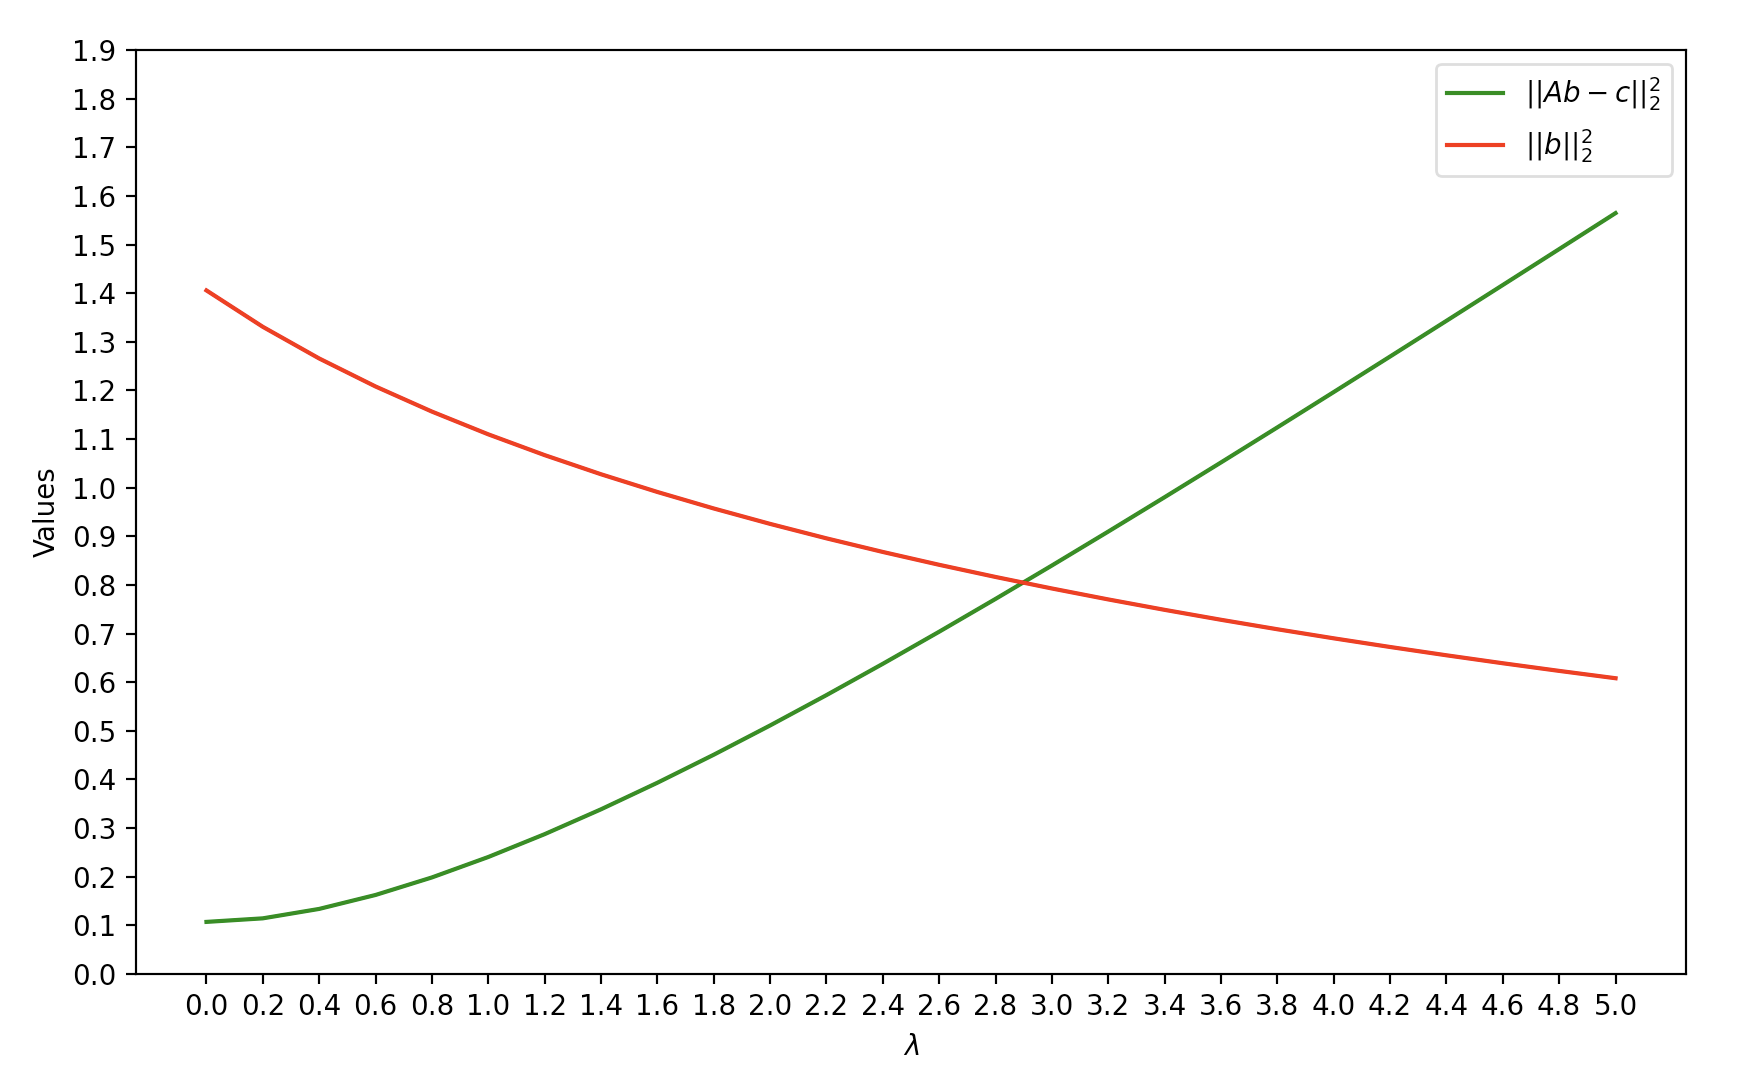
\includegraphics[scale=0.3]{img.jpg}
	\caption{figure of lambda}
	\label{figure}
\end{figure}
~\\
the solution of b is:\\

\begin{lstlisting}
	import numpy as np
	import matplotlib.pyplot as plt
	A = np.array([[1, 0, 2],[1, 1, 0],[0, 2, 1],[2, 1, 1]])
	c = np.array([2, 1, 1, 3])
	I = np.identity(3)
	b_list=[]
	o_list=[]
	x=[]
	for i in range(0, 52, 2):
		x.append(0.1*i)
		B = A.T @ A + 0.1*i*I
		X = np.linalg.pinv(B) @ A.T
		b_hat = X @ c
		M = A@b_hat-c
		b_list.append(b_hat.T @ b_hat)
		o_list.append(M.T @ M)
	plt.figure(figsize=(10,6),dpi = 100)
	plt.plot(x,o_list,color = 'green',linestyle = '-',label = r'$||Ab - c||_2^2$')
	plt.plot(x,b_list,color = 'r',linestyle = '-',label = r'$||b||_2^2$')
	plt.ylabel('Values')
	plt.xlabel(r'$\lambda$')
	plt.xticks(np.arange(0,5.2,0.2))
	plt.yticks(np.arange(0,5,0.1))
	plt.legend()
	plt.show()
\end{lstlisting}

\begin{figure}[htbp]
	\centering
	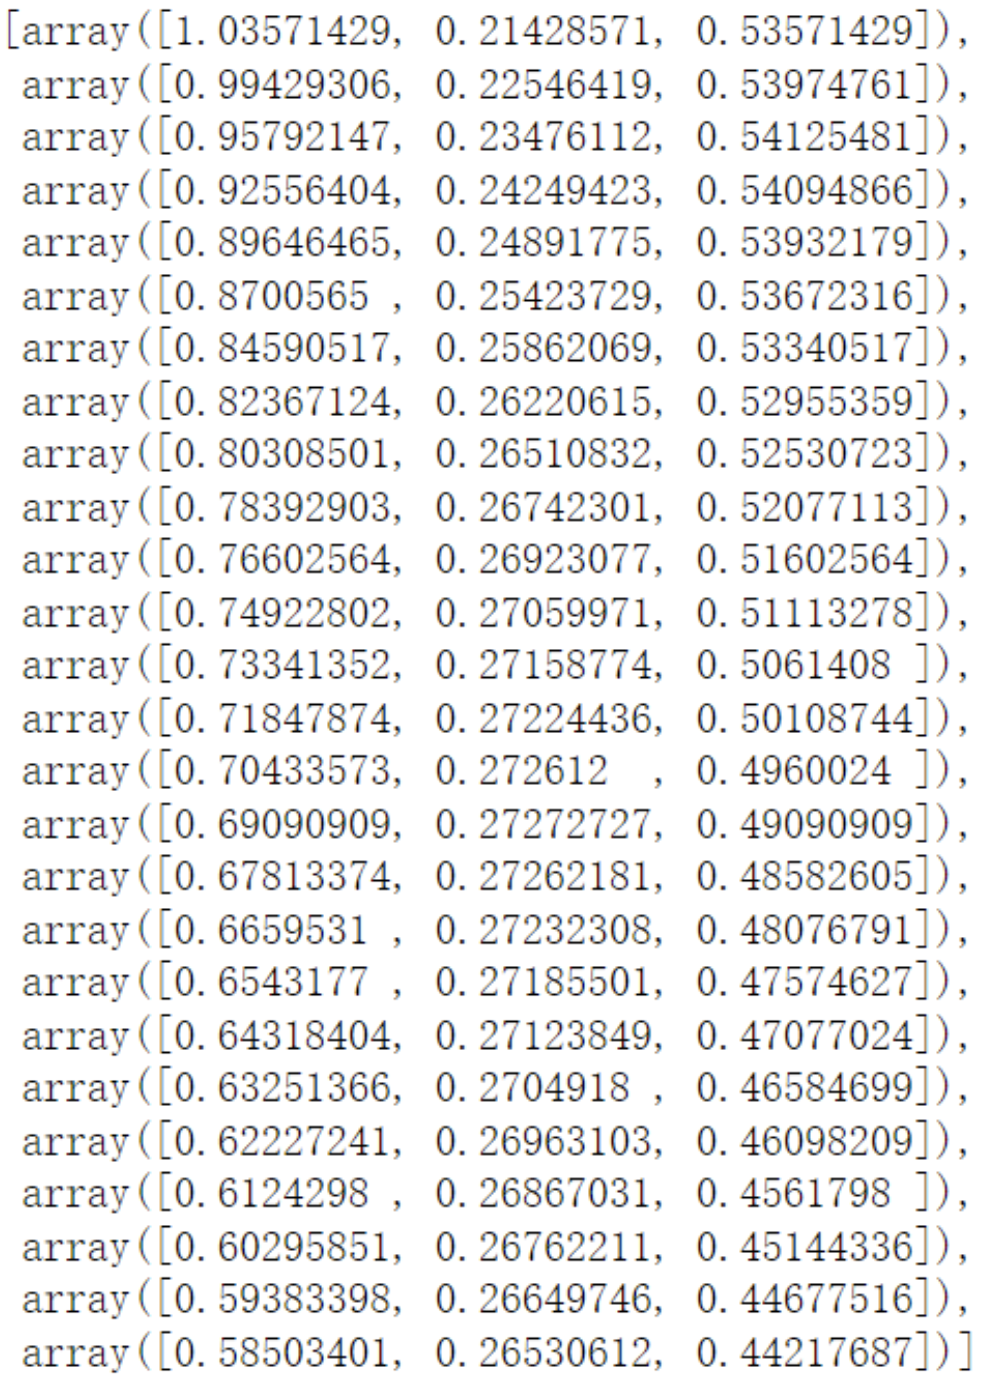
\includegraphics[scale=0.3]{img2.jpg}
	\caption{value of b}
	\label{figure}
\end{figure}

\end{document}
